\chapter{Requisiti specifici} % Main chapter title

\label{Chapter3} % For referencing the chapter elsewhere, use \ref{Chapter2} 

%----------------------------------------------------------------------------------------

% Define some commands to keep the formatting separated from the content 
% \newcommand{\keyword}[1]{\textbf{#1}}

%----------------------------------------------------------------------------------------
Il presente capitolo cerca di fornire una descrizione più dettagliata dei requisiti funzionali 
utente presentati nel capitolo 2, nonché dei requisiti non funzionali imposti. \\
\indent Anche se, in teoria, i requisiti di sistema dovrebbero semplicemente descrivere i vincoli operativi 
e non come il sistema dovrebbe essere progettato, il livello 
di dettaglio adottato ha reso impossibile escludere tutte le informazioni 
sulla progettazione.

\section{Requisiti funzionali}

Il presente paragrafo si presta a descrivere in maniera più dettagliata i casi d’uso pre-
sentati nel precedente capitolo. Per la descrizione testuale di tali casi d’uso si è deciso di adottare un formato proposto da Alistar Cockburn e chiamato \textit{template di Cockburn}. Il motivo di tale scelta è legato alla sua struttura tabellare, che facilita la comprensione
delle interazioni tra attori e sistema, offrendo una rappresentazione esaustiva di tutti
gli eventi. \\
\indent Si fa presente al lettore che le tabelle seguenti contengono riferimenti a \textit{mock-up}. Per una maggiore comprensione si raccomanda di consultare questi artefatti quando vengono citati. Questo paragrafo è suddiviso nei seguenti sottoparagrafi: \\

\begin{enumerate}
    \item \textit{Template di Cockburn}: Presentazione del \textit{template di Cockburn} applicato a un \textit{caso d'uso} significativo: \textit{Filtra issues}.
    \item \textit{Prototipazione visuale via Mock-up}: I prototipi selezionati rispecchiano fedelmente l'interfaccia utente realizzata. Ciò ha permesso di individuare agevolmente sia le incongruenze nel design grafico, sia quelle relative alla logica operativa del sistema.
\end{enumerate}

\newpage
\subsection{Template di Cockburn}

\begin{center}
    \vspace*{-1em}
    \renewcommand{\arraystretch}{2.0}
    \begin{tabular}{|p{0.25\linewidth}|p{0.10\linewidth}|p{0.43\linewidth}|p{0.22\linewidth}|}
        \hline
        \textbf{Use case \#1} & \multicolumn{3}{l|}{\emph{Filtra/Ordina issues}} \\
        \hline
        \textbf{Goal in Context} & \multicolumn{3}{p{0.71\linewidth}|}{\emph{Consente all'utente di ordinare e filtrare le issue in base a diversi criteri}} \\
        \hline
        \textbf{Preconditions} & \multicolumn{3}{p{0.71\linewidth}|}{\emph{L'utente deve possedere un proprio account}} \\
        \hline
        \textbf{Success End Condition} & \multicolumn{3}{p{0.71\linewidth}|}{\emph{Il sistema restituisce i risultati della ricerca avanzata}} \\
        \hline
        \textbf{Failed End Condition} & \multicolumn{3}{p{0.71\linewidth}|}{\emph{Il sistema non produce nessun risultato di ricerca}} \\
        \hline
        \textbf{Primary Actor} & \multicolumn{3}{l|}{Utente} \\
        \hline
        \textbf{Trigger} & \multicolumn{3}{p{0.71\linewidth}|}{\emph{L'utente clicca sul pulsante "Cerca"}} \\
        \hline
        \textbf{Main Scenario} & \textbf{Step n.} & \textbf{Utente} & \textbf{Sistema} \\
        \cline{2-4}
        & 1 & & \emph{Mostra M1} \\
        \cline{2-4}
        & 2 & \emph{Clicca sul pulsante "Cerca"} & \\
        \cline{2-4}
        & 3 & & \emph{Mostra M2} \\
        \cline{2-4}
        & 4 & \emph{Clicca sul pulsante "Filtra"} & \\
        \cline{2-4}
        & 5 & & \emph{Mostra M3} \\
        \cline{2-4}
        & 6 & \emph{Seleziona il tipo di filtro} & \\
        \cline{2-4}
        & 7 & & \emph{Mostra M4} \\
        \cline{2-4}
        & 8 & \emph{Clicca sul pulsante "Apply"} & \\
        \cline{2-4}
        & 9 & & \emph{Mostra M5} \\
        \hline
    \end{tabular}
\end{center}

% \begin{center}
% 	\vspace*{-1em}
% \def\arraystretch{2.0}

% \begin{tabular}{|p{0.3\linewidth}|p{0.7\linewidth}|}
% \hline 
% \textbf{Primary Actor} & Utente  \\
% \hline
% \textbf{Trigger} & \emph{L'utente clicca sul pulsante "Filtra/Ordina"} \\
% \hline
% \textbf{Main Scenario} &  \begin{tabular}{p{0.12\linewidth}|p{0.55\linewidth}|p{0.21\linewidth}}
%                     \textbf{Step n.} &
%                     \textbf{Utente} &
%                     \textbf{Sistema} \\
%                     \hline
%                     \end{tabular} \\
% & \begin{tabular}{p{0.12\linewidth}|p{0.55\linewidth}|p{0.21\linewidth}}
%                     1 &
%                      &
%                     \emph{Mostra M1} \\
%                     \hline
%                     \end{tabular} \\
% & \begin{tabular}{p{0.12\linewidth}|p{0.55\linewidth}|p{0.21\linewidth}}
%                     2 &
%                      \emph{Clicca sul pulsante "Filtra/Ordina"} &
%                      \\
%                     \hline
%                     \end{tabular} \\
% & \begin{tabular}{p{0.12\linewidth}|p{0.55\linewidth}|p{0.21\linewidth}}
%                     3 &
%                       &
%                      \emph{Mostra M2} \\
%                     \hline
%                     \end{tabular} \\
% & \begin{tabular}{p{0.12\linewidth}|p{0.55\linewidth}|p{0.21\linewidth}}
%                     4 &
%                      \emph{Seleziona il tipo di filtro} &
%                      \\
%                     \hline
%                     \end{tabular} \\
% & \begin{tabular}{p{0.12\linewidth}|p{0.55\linewidth}|p{0.21\linewidth}}
%                     5 &
%                      &
%                      \emph{Mostra M3} \\
%                     \hline
%                     \end{tabular} \\
% & \begin{tabular}{p{0.12\linewidth}|p{0.55\linewidth}|p{0.21\linewidth}}
%                     6 &
%                     \emph{Clicca sul pulsante "Cerca"}  &
%                     \\
%                     \hline
%                     \end{tabular} \\
% & \begin{tabular}{p{0.12\linewidth}|p{0.55\linewidth}|p{0.21\linewidth}}
%                     7 &
%                       &
%                     \emph{Mostra M4} \\
%                     \hline
%                     \end{tabular} \\
% \hline
% \end{tabular} 
% \end{center}

\clearpage

\subsection{Prototipazione visuale via Mock-up}

\begin{figure}[!ht] 
\begin{center}
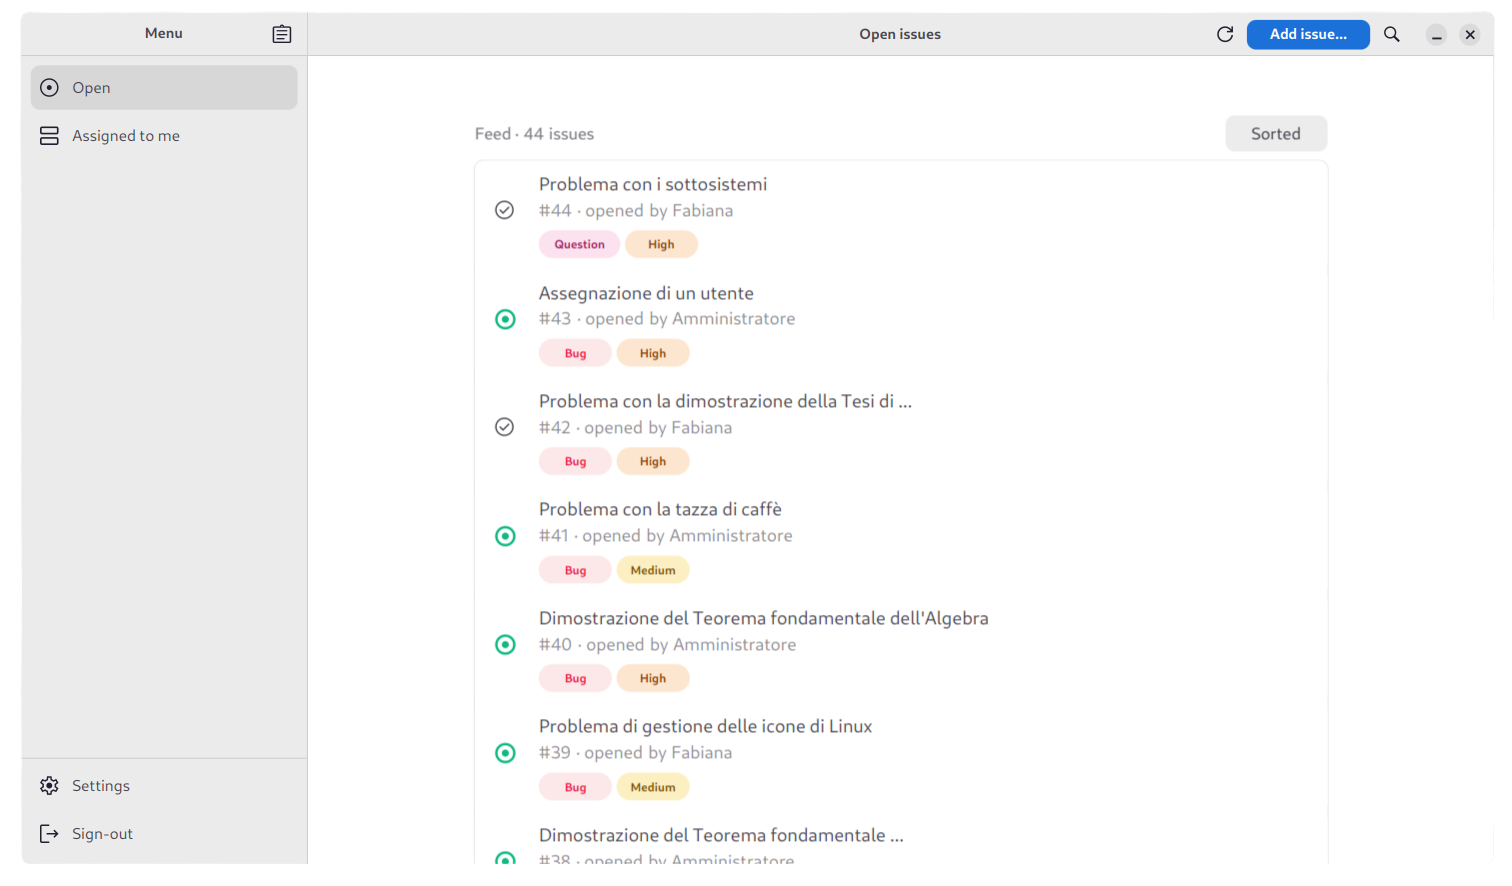
\includegraphics[width=10cm]{Chapters/Mockup-1.png}
\end{center}
\caption{Mock-up \textit{M1}}
\label{fig:f1} 
\end{figure}

\begin{figure}[!ht] 
\begin{center}
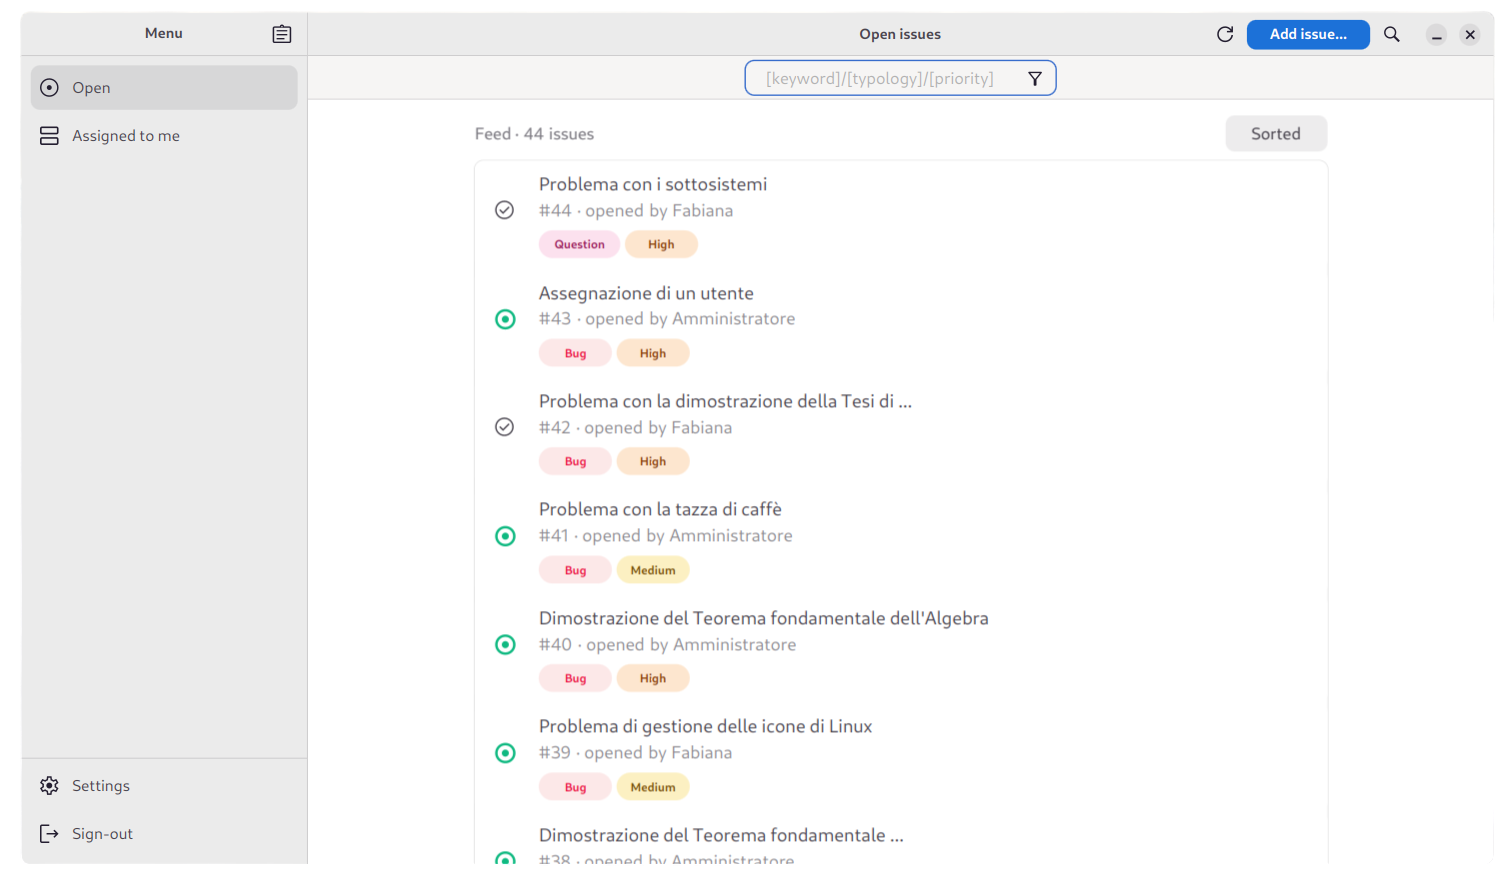
\includegraphics[width=10cm]{Chapters/Mockup-2.png}
\end{center}
\caption{Mock-up \textit{M2}}
\label{fig:f1} 
\end{figure}

\begin{figure}[!ht] 
\begin{center}
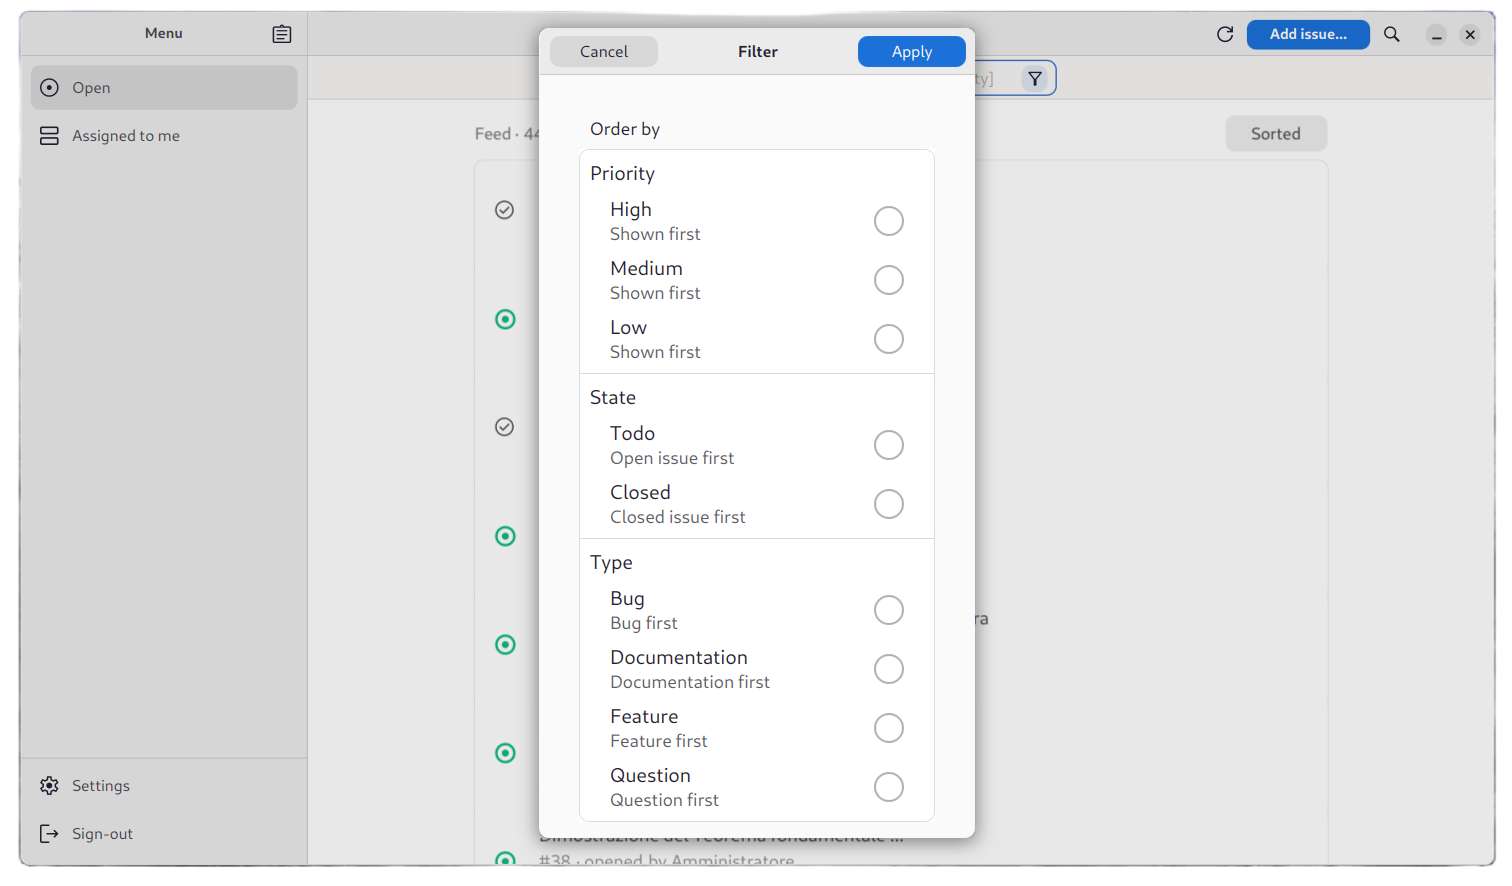
\includegraphics[width=10cm]{Chapters/Mockup-3.png}
\end{center}
\caption{Mock-up \textit{M3}}
\label{fig:f1} 
\end{figure}

\begin{figure}[!ht] 
\begin{center}
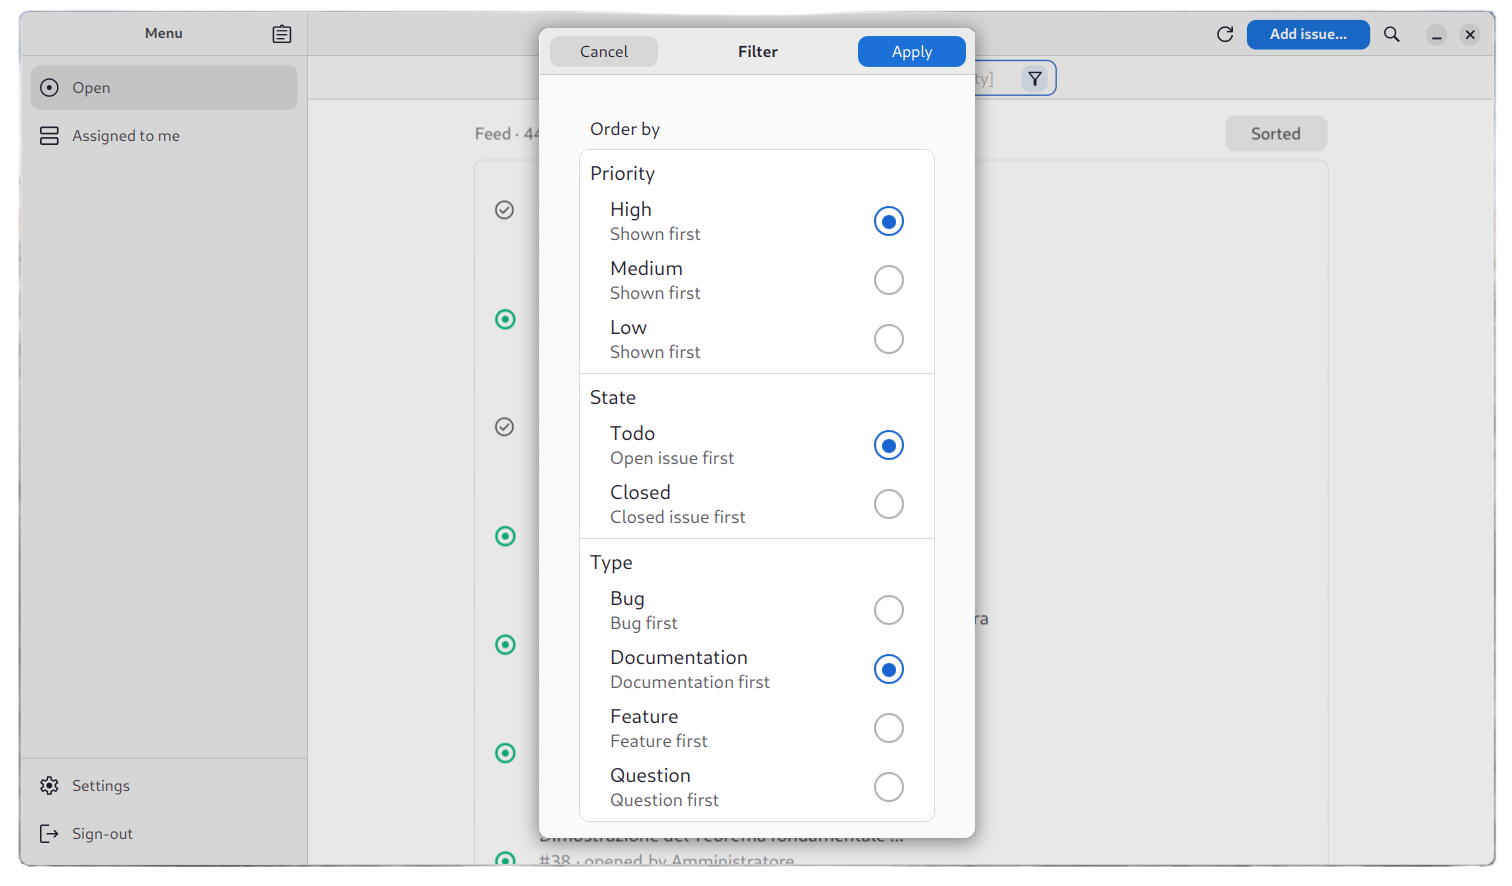
\includegraphics[width=10cm]{Chapters/Mockup-4.png}
\end{center}
\caption{Mock-up \textit{M4}}
\label{fig:f1} 
\end{figure}

\begin{figure}[!ht] 
\begin{center}
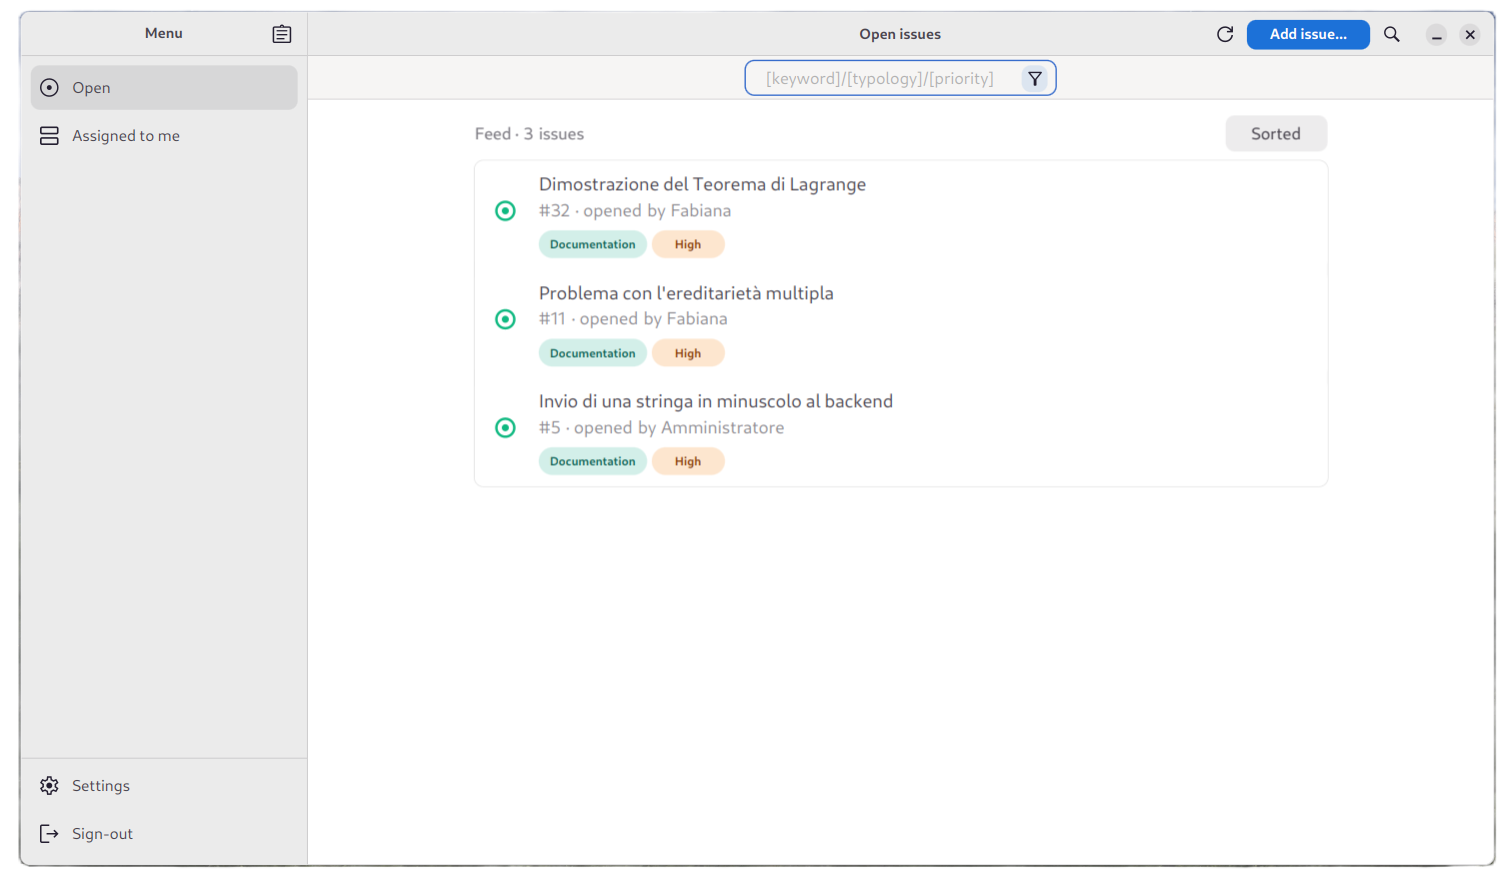
\includegraphics[width=10cm]{Chapters/Mockup-5.png}
\end{center}
\caption{Mock-up \textit{M5}}
\label{fig:f1} 
\end{figure}

\section{Requisiti non funzionali}

\subsection{Requisiti del prodotto}

\begin{quote}
\begin{enumerate}[label=\textit{RP\arabic*}]
  \item (\textit{Requisito di affidabilità}): Il sistema deve offrire un alto grado di probabilità con cui fornisca correttamente i servizi come atteso dal cliente in un determinato periodo di tempo.
  
  \item (\textit{Requisito di apprendimento}): Il sistema deve offrire un alto grado di \textit{familiarizzazione} dell'utente con le funzioni del prodotto entro un determinato periodo di tempo.

  \item (\textit{Requisito di adeguatezza}): Il sistema deve facilitare il raggiungimento dei compiti e degli obiettivi da parte dell'utente.

   \item (\textit{Requisito di portabilità}): Una parte del sistema (\textit{back-end}) può essere eseguita in ambienti diversi. Il termine ambiente può riferirsi alla piattaforma hardware o all'ambiente software.

  \item (\textit{Requisito di confidenzialità}): Il sistema deve impedire accessi non autorizzati a informazioni riservate. 
\end{enumerate} 
\end{quote}

\subsection{Requisiti organizzativi}

\begin{quote}
\begin{enumerate}[label=\textit{RO\arabic*}]
  \item (\textit{Requisito sull'architettura}): Il sistema deve basarsi su una architettura distribuita. \\
    \textbf{\textit{Requisiti di sistema:}} 
    \begin{itemize}
        \item Il sistema deve prevederre due macro-componenti indipendenti: \textit{back-end} e \textit{front-end}.
        \item Il \textit{back-end} deve essere composto da almeno una componente che gestisce la logica di business e i dati.
        \item Il \textit{back-end} deve offire una interfaccia di programmazione, con cui comunicare, mediante \textit{API REST}.
        \item Il \textit{front-end} deve comunicare con il \textit{back-end} solo tramite le \textit{API} esposte.
        \item Il \textit{front-end} deve essere realizzato come applicazione desktop, come applicazione web, oppure come applicazione mobile.
    \end{itemize} 
    
  \item (\textit{Requisito di implementazione}): Per la fase di implementazione devono essere utilizzati linguaggi di programmazione Object-Oriented. \\
  \textbf{\textit{Requisiti di sistema:}} 
    \begin{itemize}
        \item Sia il \textit{back-end} che il \textit{front-end} devono essere realizzati utilizzando linguaggi del paradigma ad oggetti.
        \item Il \textit{front-end} dovrebbe essere un'applicazione desktop realizzata con Java e le librerie grafiche Swing o JavaFX.
    \end{itemize} 
  
  \item (\textit{Requisito sugli strumenti}): In fase di produzione devono essere utilizzati tool di CASE. \\
  \textbf{\textit{Requisiti di sistema:}} 
    \begin{itemize}
        \item Strumenti come Visual Paradigm o Modelio devono essere utilizzati in fase di progettazione.
    \end{itemize}
  
  \item (\textit{Requisito di consegna}): Il prodotto software e la relativa documentazione devono essere consegnati entro il 30 Settembre 2026. \\
  \textbf{\textit{Requisiti di sistema:}} 
    \begin{itemize}
        \item Per il dettaglio completo delle scadenze di progetto si rimanda al capitolo \textbf{8} del documento \textbf{Progetto di Ingegneria del software.pdf}. 
    \end{itemize}
  
  \item (\textit{Requisito di unicità}): Il sistema deve essere progettato rispettando i requisiti antiplagio, in grado di soddisfare e superare gli standard richiesti in materia di originalità dei contenuti. \\
  \textbf{\textit{Requisiti di sistema:}} 
    \begin{itemize}
        \item Tutti gli artefatti consegnati vengono processati con software antiplagio Turnitin, e raffrontati automaticamente con progetti degli anni scorsi e di quest’anno.
    \end{itemize}
\end{enumerate} 
\end{quote}